\documentclass[sigplan,review,anonymous]{acmart}

\settopmatter{printfolios=true,printccs=false,printacmref=false}
\renewcommand\footnotetextcopyrightpermission[1]{}
\pagestyle{plain}
\raggedbottom
\setlength{\emergencystretch}{2em}

\begin{document}

\title{World-Oriented Programming: Appendix Figures}
\shorttitle{WOP Appendix}

\maketitle

\appendix
\section{Supplementary Interface Figures}

This appendix collects interface figures that are useful for talks, extended review, or supplementary material, but are not strictly necessary in the main paper narrative.

\begin{figure*}[t]
  \centering
  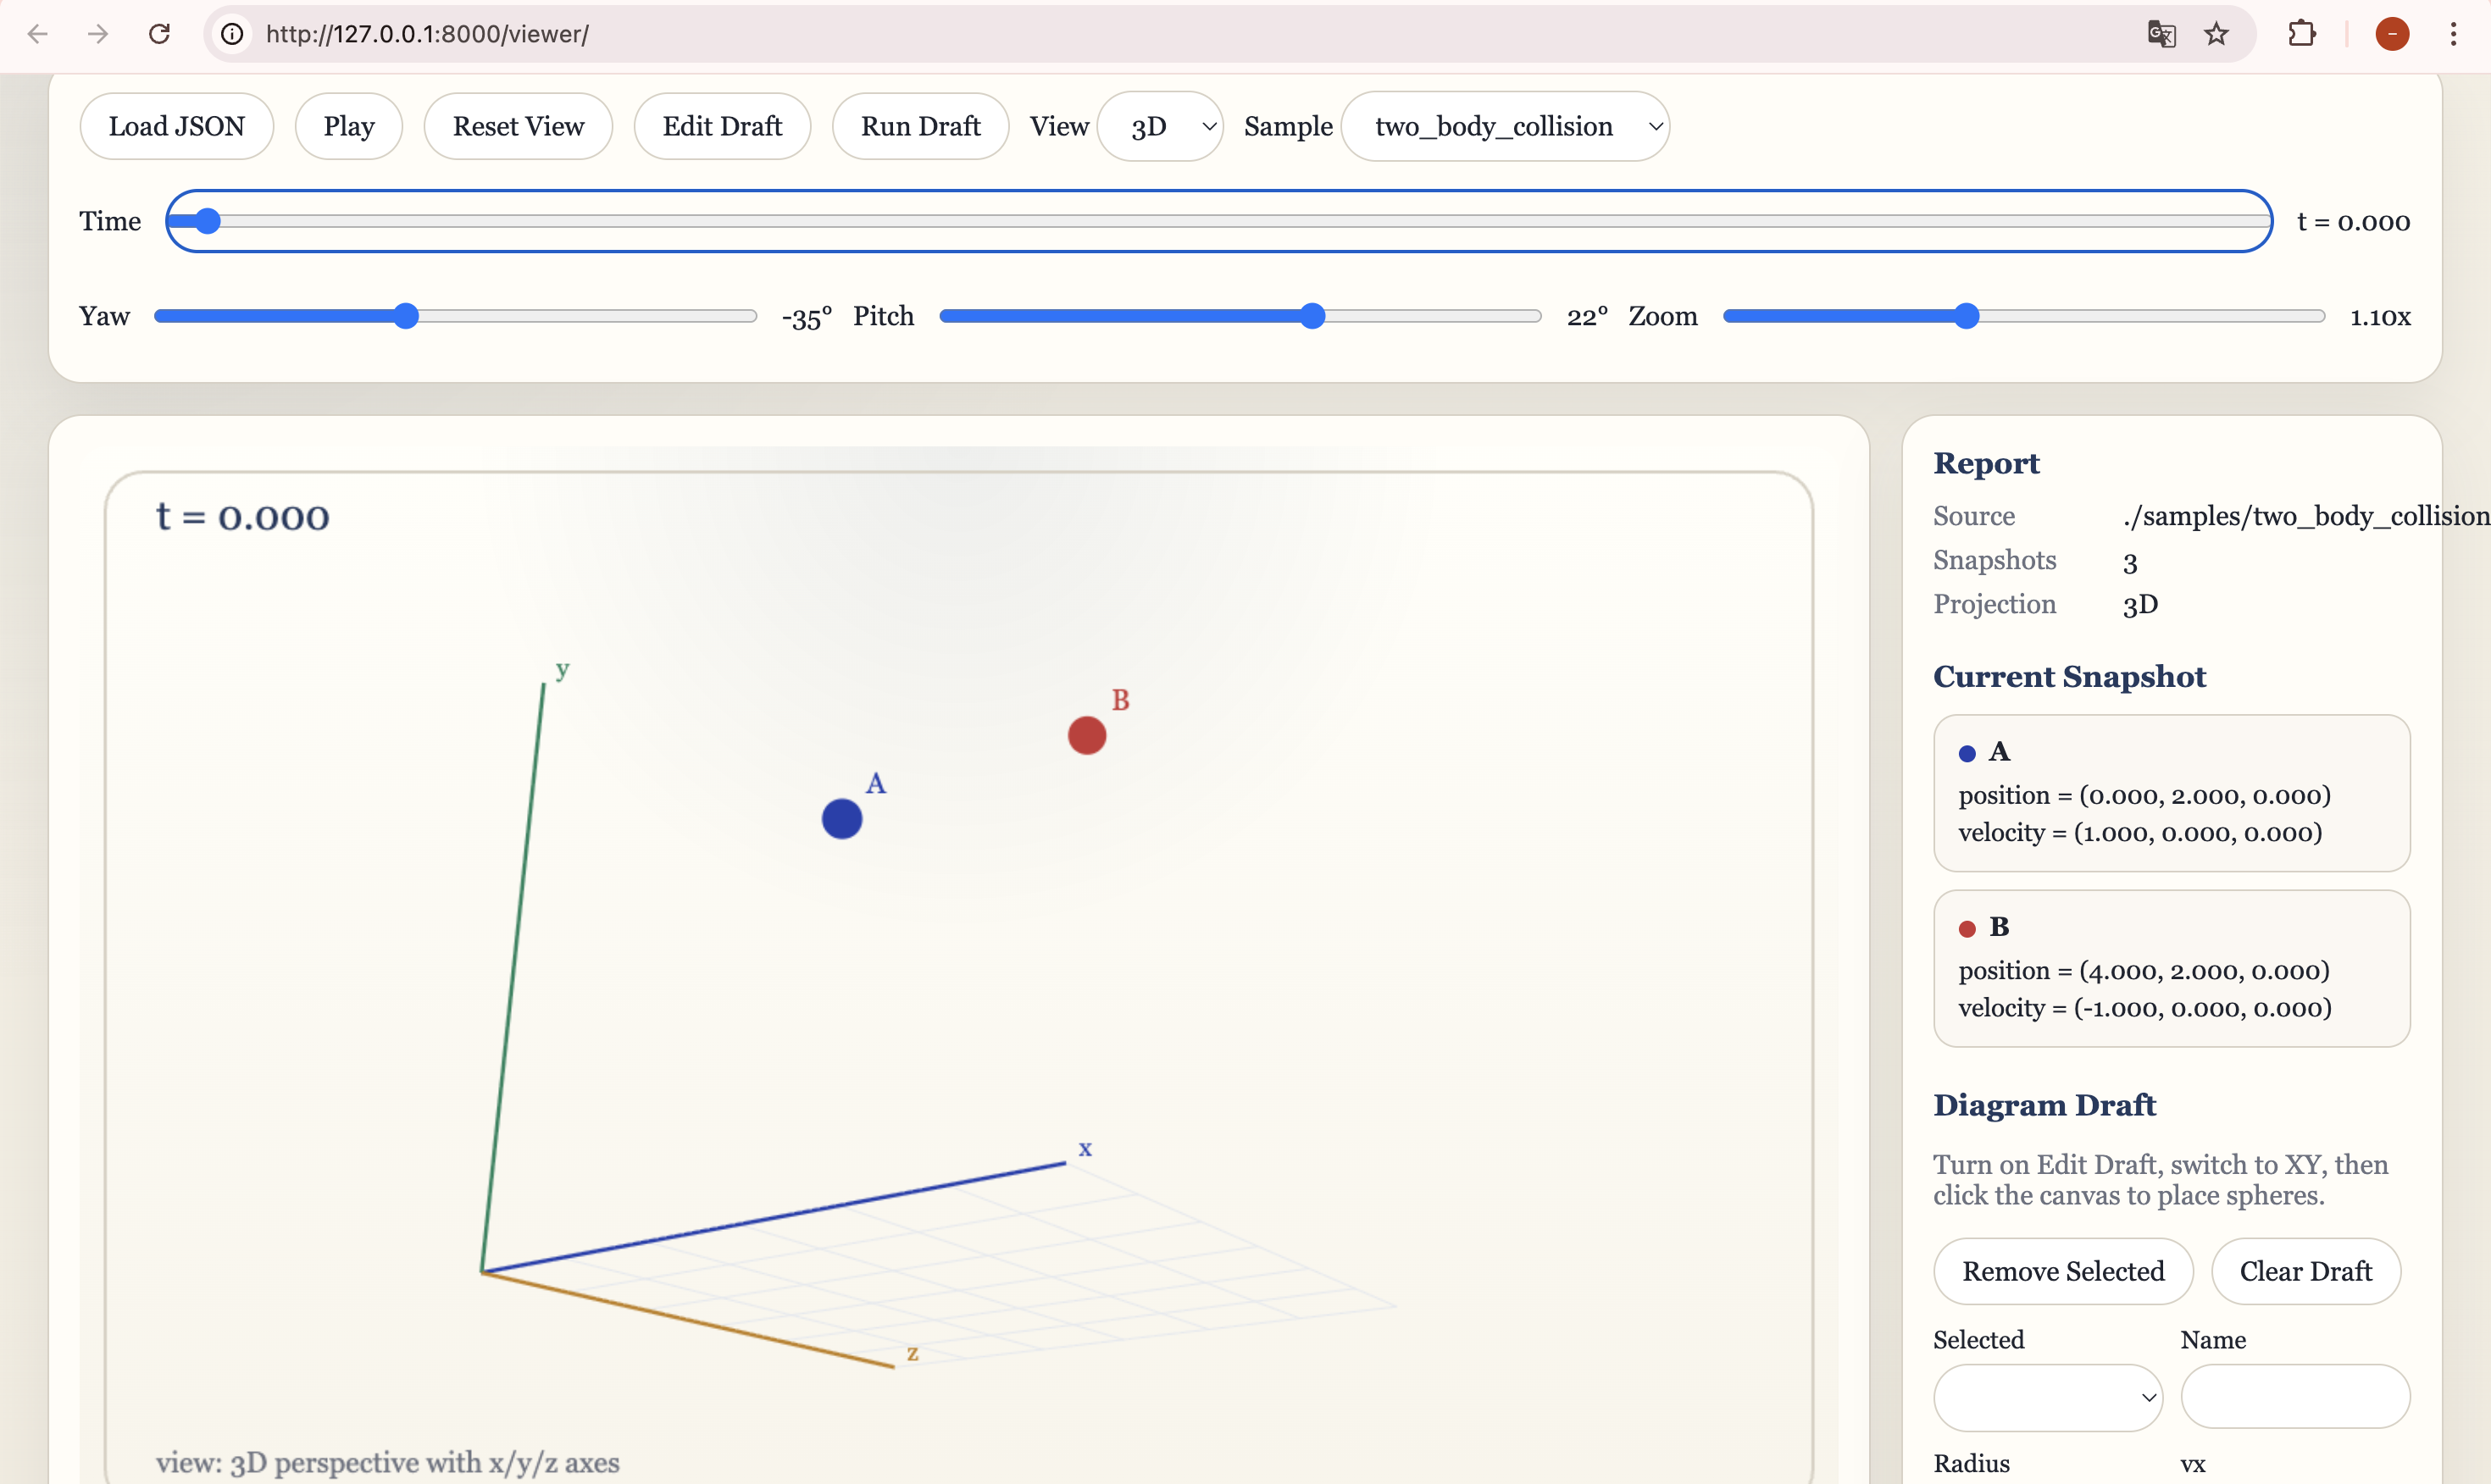
\includegraphics[width=\textwidth]{../figures/viewer-01-3d-two-body-paper.png}
  \caption{Interactive viewer overview for executable world inspection. The two-body collision example is shown in the browser-based \texttt{sekai} viewer, where one world report can be inspected spatially, temporally, and structurally without a separate viewer pipeline.}
  \label{fig:appendix-viewer-overview}
\end{figure*}

\begin{figure*}[t]
  \centering
  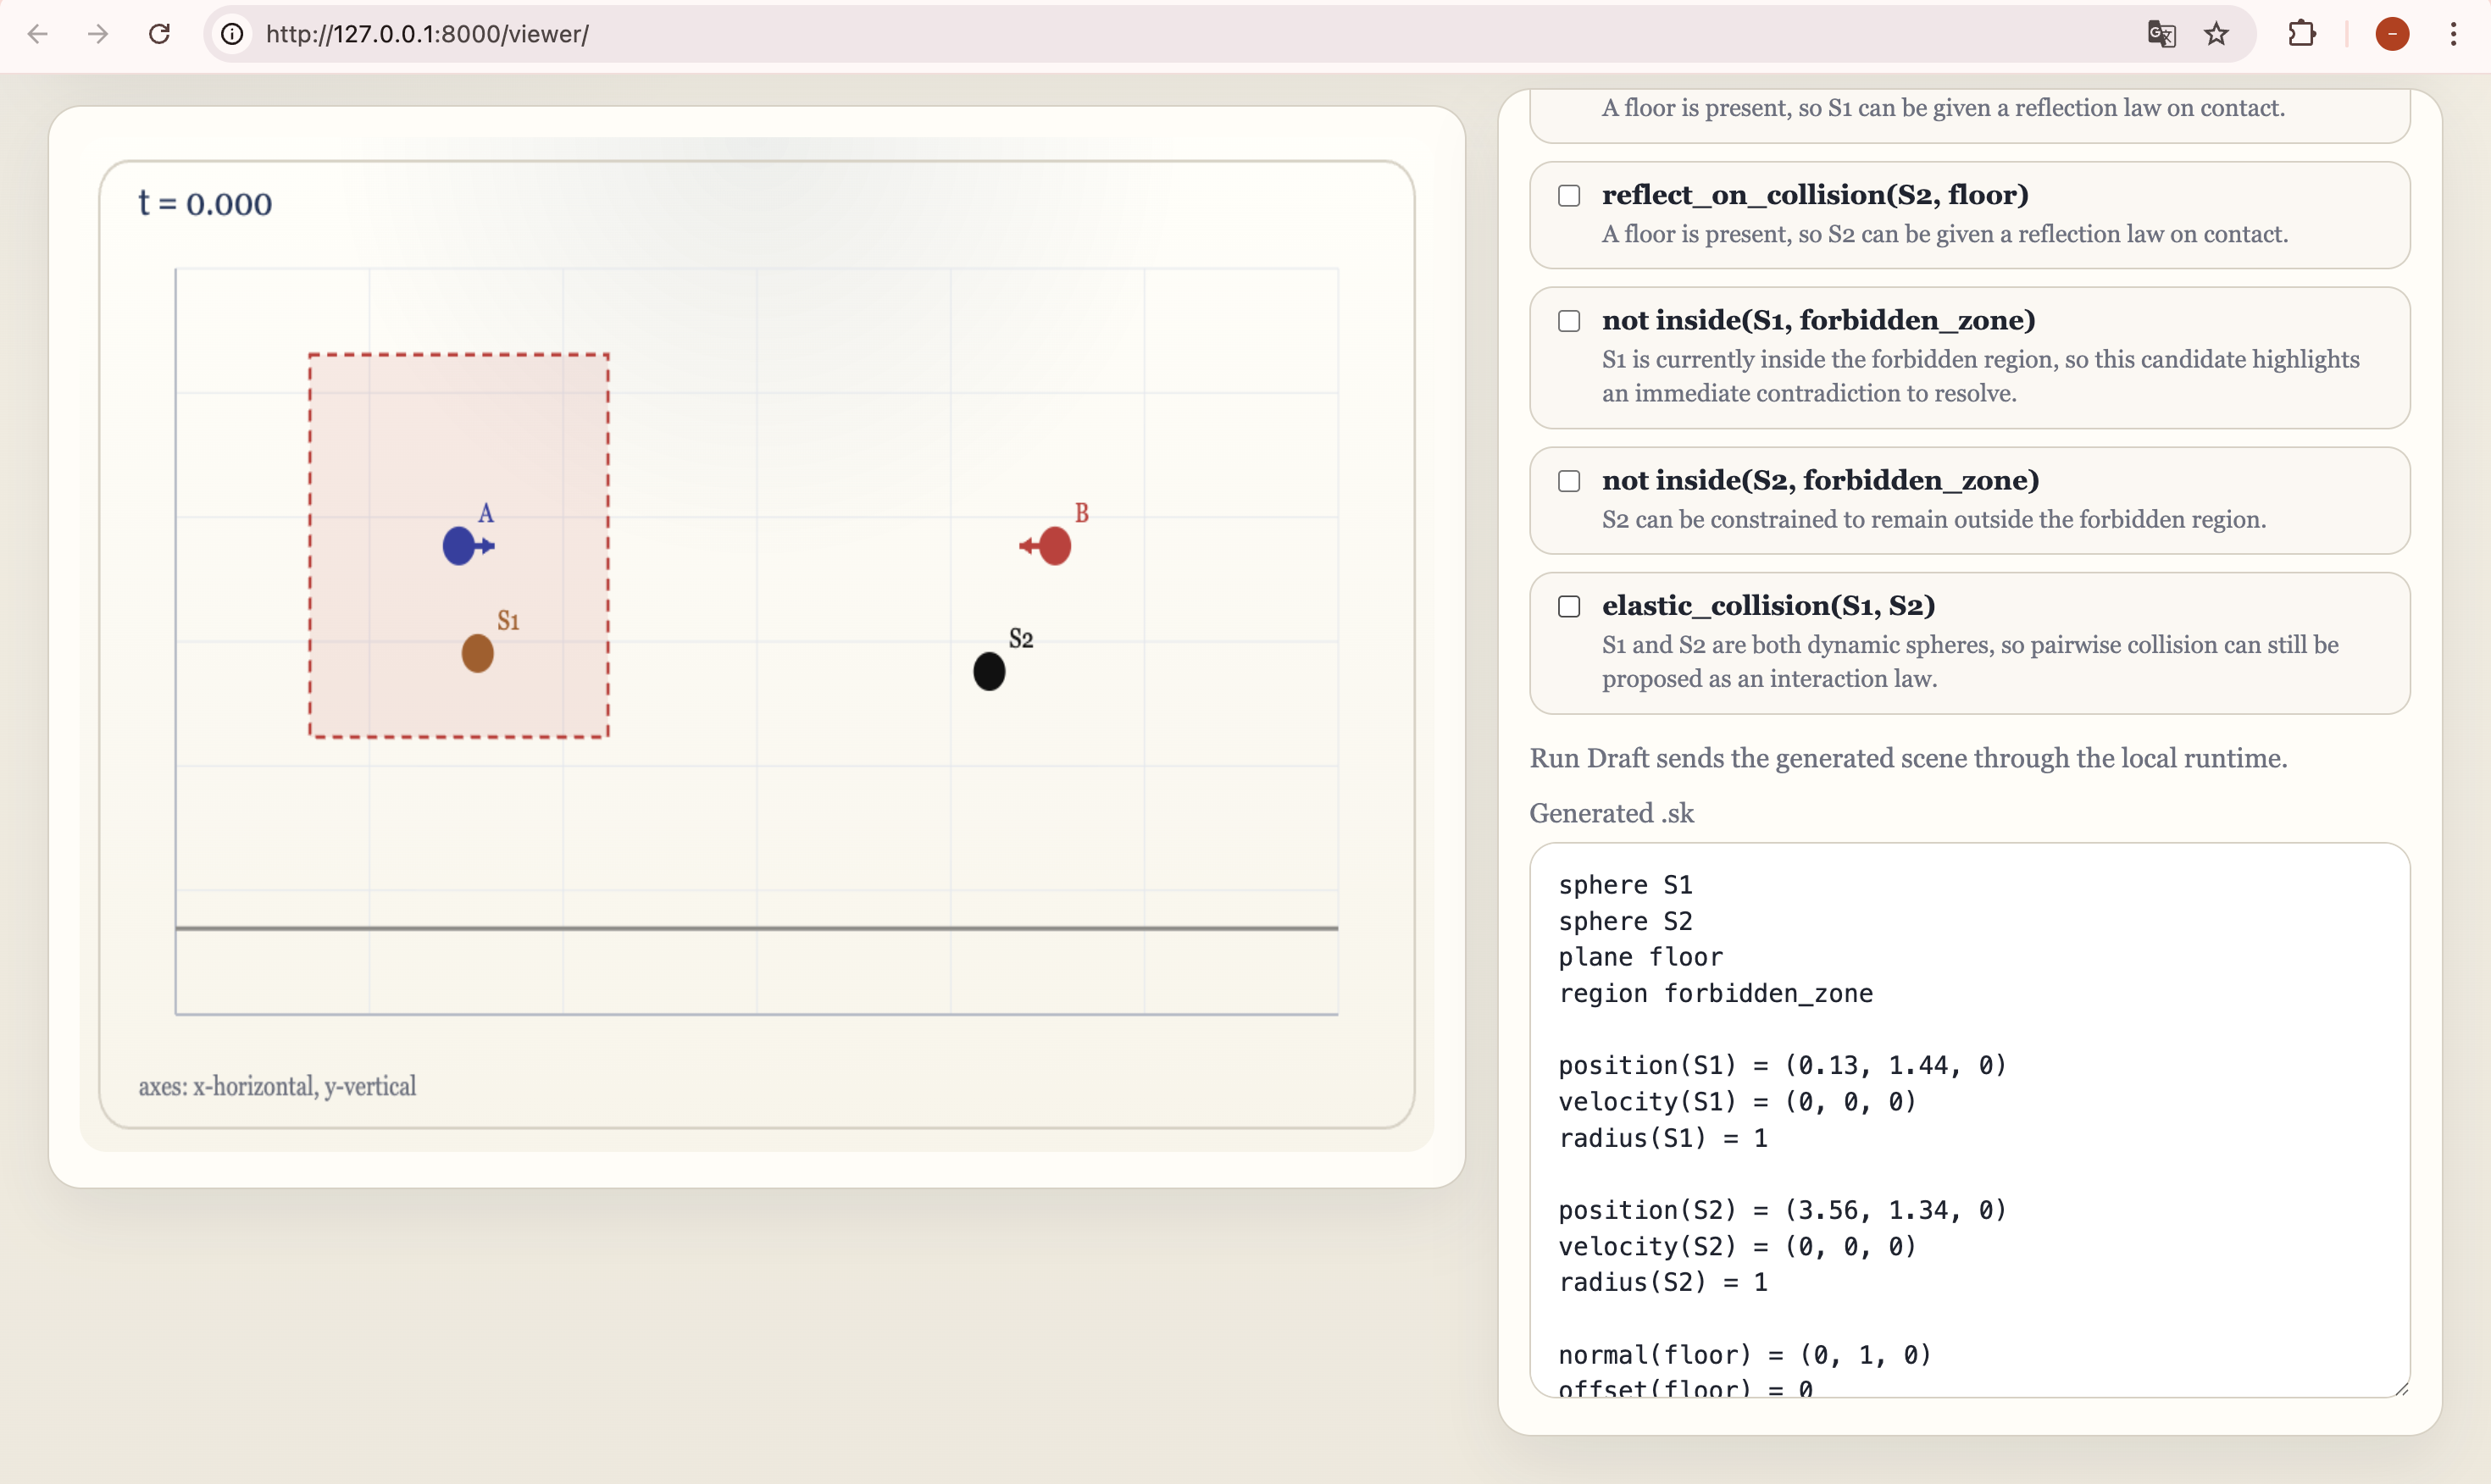
\includegraphics[width=\textwidth]{../figures/viewer-02-draft-candidates-paper.png}
  \caption{Diagram-to-logic candidate generation in the draft editor. Two placed spheres and a forbidden region give rise to proposed world laws such as floor reflection, forbidden-region exclusion, and pairwise collision.}
  \label{fig:appendix-viewer-candidates}
\end{figure*}

\end{document}
